\documentclass[twocolumn,10pt]{article}
\usepackage[a4paper, top=0.5in, bottom=0.6in, left=0.5in, right=0.5in]{geometry}

\usepackage{graphicx}
\usepackage{algorithm}  
\usepackage{algorithmicx}  
\usepackage{algpseudocode}  
\usepackage{amsmath}
\usepackage{url}
\usepackage{xcolor}
\usepackage{listings}
\usepackage{enumitem}

\algnewcommand{\LeftComment}[1]{\Statex \(\triangleright\) #1}

\renewcommand{\algorithmicrequire}{\textbf{Input:}}  
\renewcommand{\algorithmicensure}{\textbf{Output:}}  
\graphicspath{{figure/}}

\begin{document}

\title{\bf Grouper: a Framework for Developing Mobile Applications using a Secret Sharing Scheme and Untrusted Servers}

\author{
	Meng Li and Yasushi Shinjo \\
	University of Tsukuba
}

\maketitle

\begin{abstract}

This paper presents Grouper, a framework for developing mobile applications.
Grouper uses a secret sharing scheme to create several shares from a marshalled object and uploads these shares to multiple untrusted servers. 
These untrusted servers construct a self-destruction system.
Uploaded shares will be deleted after a period of time.
Mobile devices exchange messages via untrusted servers based on the Grouper Message Protocol.
We have implemented the Grouper framework for iOS, macOS, tvOS and watchOS in the Objective-C language.
It consists of a client framework and a Web service.
We have implemented three applications using Grouper: an iOS application Account Book and a benchmark application Test.
We evaluate the development efforts and the performance of Grouper. 
Experimental results show that the performance of Grouper is feasible for mobile applications that are used in a small group of people.

\end{abstract}

\textbf{Keywords: mobile application security, secret sharing, untrusted server}

\section{Introduction}

People use mobile applications everyday. 
Conventional mobile applications are built based on a client-server mode and require central servers for storing shared data and processing confidential information.
When users use such mobile applications, they must fully trust the central servers.
If the central servers are accessed by an attacker, a curious administrator or a government, private information will be revealed because data is often stored on the central servers in cleartext. 
In addition, users may lose their data when service providers shut down their servers.

To address this problem about using central servers, Vanish\cite{geambasu2009vanish}, SafeVanish\cite{zeng2010safevanish}, SeDas\cite{zeng2012sedas} and CouldSky\cite{zeng2015cloudsky} construct a data self-destruction system as their cloud storage.
In these approaches, servers store data temporarily and delete data after a period of time.

These existing approaches have following problems.
Firstly, they do not support data recovery when some nodes miss getting data from shared storage.
Application developers have to deal with such cases by themselves.
Secondly, these approaches do not support developing general mobile applications.

To address these problems, we are developing Grouper, a framework for developing mobile applications. 
Grouper provides object synchronization among mobile devices.
In Grouper, a sender node translates an updated object into shares using a secret sharing scheme and uploads these shares to untrusted servers. 
A receiver node downloads some of these shares and reconstructs the object.
The untrusted servers construct a self-destruction system, and delete these shares after a period of time.
Unlike existing approaches, although Grouper uses the data self-destruction scheme, it supports data recovery when some nodes miss getting shares from untrusted servers.
When a receiver node misses getting shares, the Grouper framework automatically asks the sender to upload missing shares again.
This ensures reliable data sharing among devices of a group.
In addition, data can be recovered even untrusted servers shut down because all devices of a group keep a complete data set of this group.

Grouper consists of a client framework and a Web service.
We have implemented the Web service running on the multiple untrusted servers in Java. 
We have embedded a Sync framework in Grouper to synchronize objects among mobile nodes.
We have implemented two applications using Grouper: an iOS application Account Book and a benchmark application Test.
These implementations show that Grouper makes it easy to develop mobile applications with data synchronization.

The contributions of this paper are as follows.
Firstly, we provide support for data recovery when some nodes miss getting data from untrusted servers.
Grouper realizes reliable data synchronization among nodes using a reliable multicast technique.
Secondly, we make it easier to develop mobile applications.
A developer can add data synchronization functions to stand alone applications with a few lines of code.

\section{Threat Model}

In this section, we introduce the assumptions and threat model underlying the Grouper framework.
We target mobile applications that are used in a small group of people.
A group consists of an owner and other members.
Each member has a mobile device.
A owner invites other members in a face-to-face way.

Firstly, server are a passive adversary, and can read all data, but it does not actively attack.
Servers host Web services and perform device authentication.
Servers generate access keys for group members. 
When a device wants to get/put data from/to untrusted servers, the device sends a request with an access key.
In this paper, we do not address other types of attacks such as user tracking and metadata collection by servers. 
For example, servers can track users with IP addresses, and Grouper cannot hide social graphs against such tracks.

Secondly, data transportation between a device and an untrusted server is secure.
We can protect it using Transport Layer Security (TLS) or other encryption techniques.
Grouper focuses on privacy in the data storage of servers rather than data transportation.

Thirdly, in an application, all group members are not malicious and their devices connect to each other securely in a face-to-face distance.
We target applications that are used in a small group at the user invitation time.
For example, the group members are working in an office.
They know one another and they are not malicious.
When a group owner invites new members, the owner authenticates group members by a face-to-face way.

At last, a server is isolated from one another and managed by independent providers.
We assume that providers of untrusted servers do not expose users' data to other providers.
For example, a group owner can pick up servers of Amazon, Google, and Microsoft, which are supposed not to expose users' data to other cloud providers.

\section{Design}

This section describes the design of the Grouper framework.

\subsection{Overview}

Our goal is to support developing mobile applications that are not relying on trusted central servers.

To achieve this goal, we provide the Grouper framework.
This framework provides the following functions:

\begin{itemize}
	\setlength{\itemsep}{1pt}
	\setlength{\parskip}{0pt}
	\setlength{\parsep}{0pt}
	\item \textbf{Data Synchronization.} 
	If an user updates or deletes an object in his device, the mirrors of this object in other devices are updated or deletes.
	\item \textbf{Group management.} 
	A group owner can create a group and invite other members to his group.
\end{itemize}

For example, \emph{Account Book} is an iOS application developed using Grouper. 
In this application, a leader of a small company creates a group and invites employees to the group. 
Then, the employees can record the income and expenditure of this company.
These income and expenditure records are represented as objects and shared among devices.
Anyone can edit and delete existing records.

Grouper uses untrusted servers to exchange messages among mobile devices.
Untrusted servers construct a self-destruction system, and delete messages after a period of time.
We call it a Time To Live(TTL).

Grouper protect messages from the providers of untrusted servers using a secret sharing scheme.
Grouper uses Shamir's secret sharing scheme to protect user data.
In  Shamir's secret sharing scheme, a member securely shares a secret with other members by generating $n$ shares using a cryptographic function\cite{smith2013layered}. 
At least $k$ or more shares can reconstruct the secret, but $k-1$ or fewer shares output nothing about the secret\cite{pang2005new}. 
We describe this scheme as a function ${f(k, n)}$, where $n$ is the number of all shares, and $k$ is the threshold to combine shares. 

Grouper has the following advantages over conventional systems using untrusted servers.
Firstly, it is easy for a developer to recover from message losses in untrusted servers (Section 3.4).
Grouper performs retransmission when some mobile devices miss getting messages from untrusted servers.
Developers of mobile applications do not have to specify lifetimes of messages.
Secondly, it is easy for a group owner to invite other members using a safe communication channel in a face-to-face distance (Section 3.7).

\subsection{Architecture}

\begin{table*}[t]
	
	\centering
	\caption{Client API of Grouper.}
	\label{my-label}
	\begin{tabular}{ll}
		\hline
		\textbf{Method} & \textbf{Description} \\ \hline
		grouper.\textbf{setup}(appId, dataStack) & 
		\begin{tabular}{@{}l@{}}
			An application invokes this method to initialize Grouper with appId and dataStack.\\
			AppId is a unique ID of an application. Datastack is used by the synchronization\\
			plugin.
		\end{tabular}  \\ \hline
		grouper.sender.\textbf{update}(object) & 
		\begin{tabular}{@{}l@{}}
			An application invokes this method after creating a new object or modifying an\\ 
			existing object. Grouper performs updating asynchronously and sends an update\\ 
			message to other devices.
		\end{tabular} \\ \hline
		grouper.sender.\textbf{delete}(object) & 
		\begin{tabular}{@{}l@{}}
			An application invokes this method when the application wants to delete an existing\\ 
			object. Grouper will delete the object and remove it in the persistent store of a\\ 
			device automatically after sending a message to other devices.
		\end{tabular} \\ \hline
		grouper.receiver.\textbf{receive}(callback) & 
		\begin{tabular}{@{}l@{}}
			An applications invokes this method to register the callback function that is called\\ 
			after Grouper processes received messages and update objects according to the\\ 
			messages. The application can use this callback function to update the user screen. 
		\end{tabular} \\ \hline
		grouper.sender.\textbf{confirm}() & 
		\begin{tabular}{@{}l@{}}
			An application needs to invoke this method periodically or occasionally to send\\ 
			a confirm message to other devices.
		\end{tabular} \\ \hline
	\end{tabular}
\end{table*}

\begin{table*}[t]
	\centering
	\caption{The API of the synchronization plugin.}
	\label{my-label}
	\begin{tabular}{ll}
		\hline
		\textbf{Method} & \textbf{Description} \\ \hline
		marshall(o) & Marshalls the object o and returns the marshalled byte array. \\
		updateRemote(b) & Unmarshalls the byte array b to the object and puts the object into the persistent store. \\ 
		deleteRemote(b) & Deletes the object in the byte array of object IDs.\\ \hline
	\end{tabular}
\end{table*}

\begin{figure}[t]
	\centering
	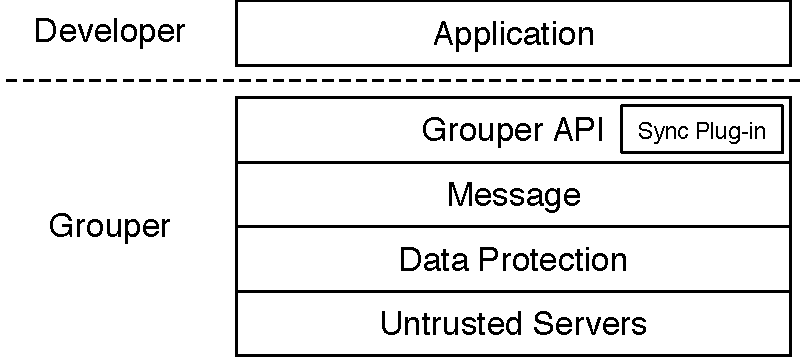
\includegraphics[scale=0.45]{architecture}
	\caption{Architecture of Grouper.}
\end{figure}

Figure 1 describes the architecture of the Grouper framework. 
An application using Grouper consists of the four following layers and a plugin:

\begin{itemize}
	\setlength{\itemsep}{1pt}
	\setlength{\parskip}{0pt}
	\setlength{\parsep}{0pt}
	\item \textbf{Grouper API.}
	A developer develops an application without data synchronization at first. 
	He adds the synchronization function to his application by using this API.
	\item \textbf{Synchronization Plugin.} 
	Grouper uses a third-party framework for data synchronization.
	This plugin marshalls an updated object in a local persistent store and the Grouper API layer passes the marshalled message to the lower reliable message layer.
	When this layer receives a message, this layer unmarshalls the message using the plugin, reconstructs an object, and puts the object into the persistent store.
	\item \textbf{Message.}
	This layer provides a message service with multicasting capability among devices.
	The destination of a massage is not only the node identifier (ID) of a single device but also "*", which means delivering to all the other nodes.
	This layer does not ensure the message delivery to other devices.
	\item \textbf{Data Protection.}
	Grouper protects user data by a secret sharing scheme in this layer.
	This layer divides a message into several shares, and uploads these shares to untrusted servers.
	When this layer downloads shares from untrusted servers, it recovers the original message using the secret sharing scheme.
	\item \textbf{Untrusted servers.}
	When a mobile device uploads a share to an untrusted server, this server receives it and stores it into a database.
	When a mobile device downloads a share from an untrusted server, this server retrieves it from the database and sends it into the device.
	An untrusted server performs device authentication using device keys.
\end{itemize}

The following subsections describe details of these layers from the top layer to the bottom layer.

\subsection{Grouper API}

The Grouper framework provides object synchronization among mobile devices through a simple client API.
A developer can add object synchronization functions to a standalone application with a few lines of code.
Table 1 shows the client API of Grouper.
An application initializes the framework by invoking the method $grouper.setup()$.
When the application needs to update an object in all devices, the application invokes the method $grouper.sender.update()$.
When the application needs to delete an object in all devices, the application invokes the method $grouper.sender.delete()$.
The the application uses the method $grouper.receiver.receive()$ to register a callback function.
This callback function is called when another node updates an object and its local mirror has been updated.
The application can use this callback function to change the values that are shown in a user interface screen.
The method $grouper.confirm()$ is used for realizing reliable messaging.
We will describe reliable messaging in Section 3.4.

The Grouper API layer relies on two modules: the synchronization plugin and the messaging layer.
When an object is updated in a local device, the synchronization plugin marshalls an updated object and returns a message.
Next, the Grouper API layer sends this messages using the messaging layer.
When an object is updated in another device, the Grouper API layer receives a message using the messaging layer.
Next, the Grouper API layer updates the object by passing the received message to the synchronization plugin.

We have not implemented the synchronization plugin by ourselves, but we make this module pluggable.
This is because there are many such synchronization modules that provide various features, and application requirements also vary.
Each application developer should choose a suitable module based on a consistency model and other requirements.
As described in Table 2, the synchronization plugin should provide the functions $marshall(o)$, $updateRemote(b)$ and $deleteRemote(b)$.
Grouper invokes them to get marshalled data from the persistent store and save unmarshalled data into the persistent store.

Because we implement our client framework in Objective-C at first, we use the Sync framework\cite{sync} to implement a data synchronization plugin currently.
The Sync framework marshalls objects into JavaScript Object Notation (JSON) strings and provides a consistency model where the newest edition wins.

\subsection{Reliable Message Delivery}

Grouper realizes reliable message delivery in the Grouper API layer over the self-destruction system.

To design this, we use a reliable multicasting technique in distributed systems\cite{tanenbaum2007distributed}.
In this reliable multicasting technique, each message has a sequence number for each sender.
Each member keeps the newest sequence numbers for senders and detects missing messages.
If a member notices missing a message from a sender, the member asks the sender to resend the update message.
For example, consider that a sender sends update message No.3 to all other members using a multicast address.
When a member receives this update message No.3, the member compares the sequence number 3 with the newest sequence number of the sender.
If the the newest sequence number of the sender is 1, this means the member missed update message No.2.
The member asks the sender to resend update message No.2.
The sender will send update message No.2 to the asked member using a unicast address.

This basic reliable multicasting technique works well for continuous medias, such as video streaming in Internet communication.
However, this does not work if receivers become often offline for a long time and servers delete messages soon.

To address this problem, we extend the basic reliable multicasting technique.
We use a special type of messages that include active sequence numbers.
Using these messages, a receiver can easily know missing messages.
We call this type of messages confirm messages.

\begin{figure}[t]
	\centering
	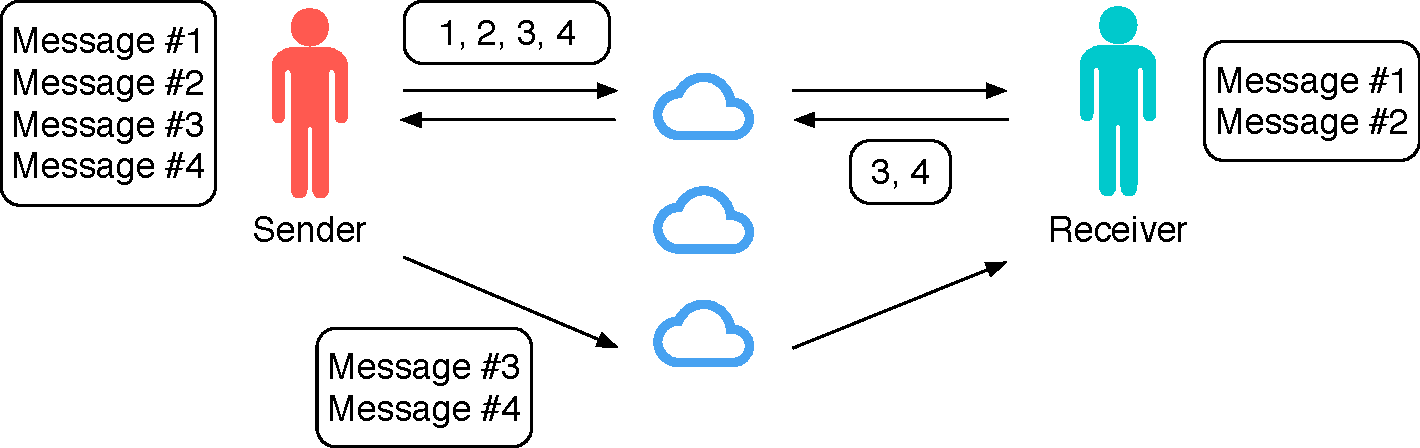
\includegraphics[scale=0.38]{reliable_sync}
	\caption{Implementing reliable messaging with continuous sequence numbers.}
\end{figure}

Figure 2 shows that the sender is sending five update messages from No.1 to No.5 to the receiver.
The sender uploads two messages, No.1 and No.2,  using a multicast address.
The receiver downloads these two messages and becomes offline.
The servers delete these two messages.
The sender uploads next three update messages from No.3 and No.5  using a multicast address.
The receiver becomes online, but the receiver does not notice that the receiver has missing messages soon.
At this time, the sender sends a confirm message that includes the newest active sequence number, 5.
The receiver receives this sequence number and compares it with the newest sequence number in the persistent store.
In Figure 3, the receiver notices that update messages No.3, No.4 and No.5 are missing.
The receiver asks the sender to resend update messages No.3, No.4 and No.5.
The sender will send update messages No.3 and No.4 to the receiver again using a unicast address.

This idea is inspired from the checkgroups message of Usenet\cite{usenet}.
In Usenet, the list of active newsgroups is maintained with two basic messages: newgroup and rmgroup.
When a node receives a newgroup message, the node adds the newsgroup to the list.
When a node receives a rmgroup message, the node removes the newsgroup from the list.
These basic messages can be lost and the list can be obsolete.
Ckeckgroups messages supplement these basic messages.
A checkgroups message includes the list of all newsgroups in a newsgroup hierarchy.
A checkgroups message is distributed periodically or after some time after basic messages are distributed.

\subsection{Unreliable Messaging Using Untrusted Servers}

This subsection describes the design of unreliable messaging in the layers of Messaging, Data Protection, and Untrusted Servers.

In these layers, we use a secret sharing scheme and multiple untrusted servers as shown in Figure 3.
In this figure, the messaging layer in the sender is sending a message to that in the receiver.

At first, this layer calls the data protection layer and creates three shares by a secret sharing scheme.
Next, this layer uploads those shares to three untrusted servers.
Each untrusted server receives one of these shares and stores it into a database.

\begin{figure}[t]
	\centering
	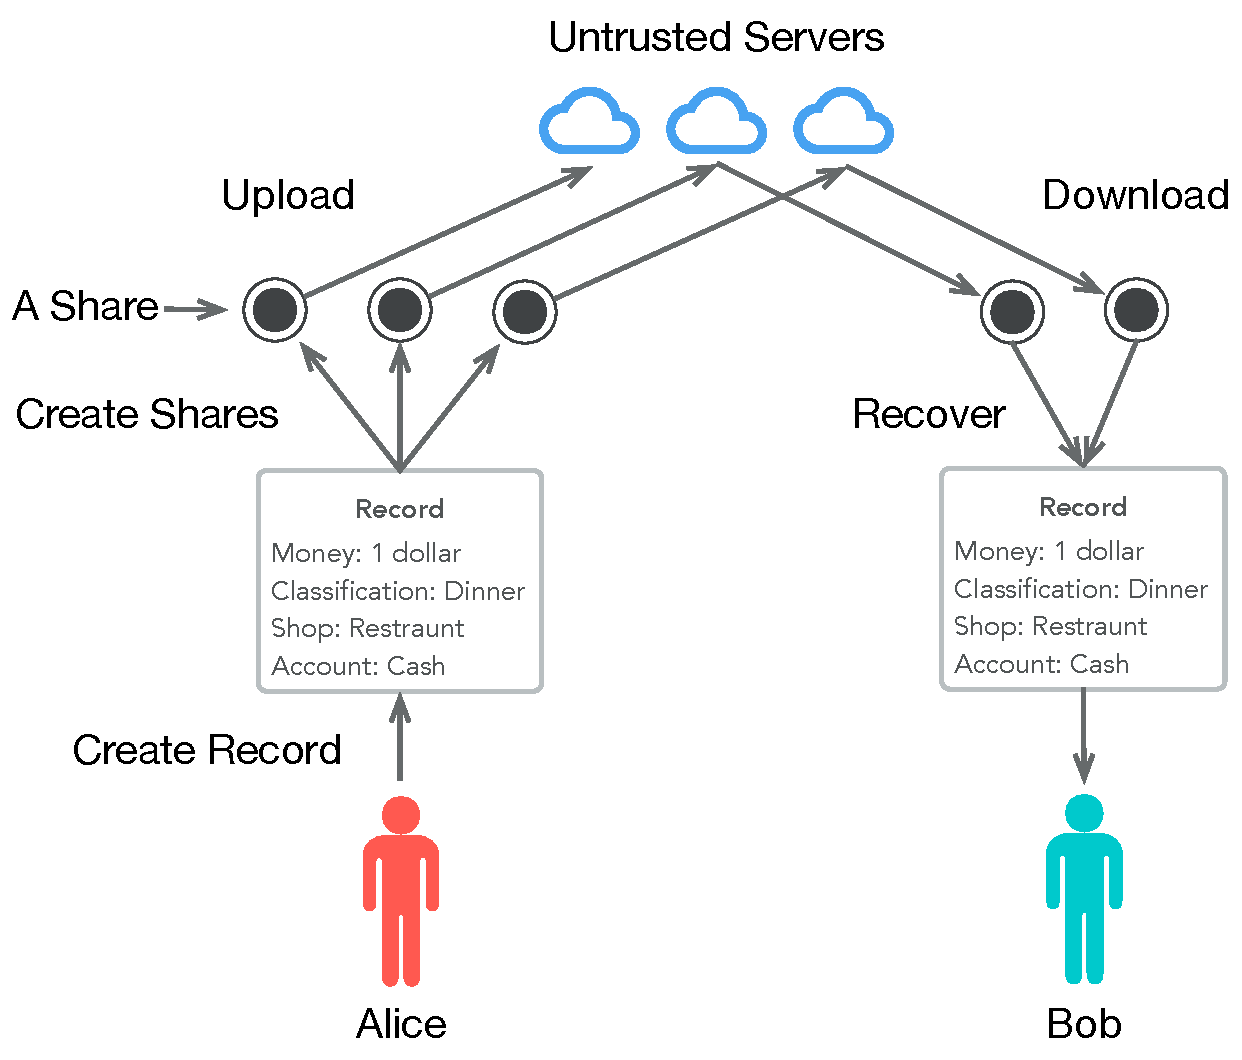
\includegraphics[scale=0.42]{sync_flow}
	\caption{Implementing unreliable messaging with a secret sharing scheme and multiple untrusted servers.}
\end{figure}


\subsection{Parameters of Secret Sharing Scheme}

The data protection layer uses the Shamir's secret sharing scheme $f(k, n)$ introduced in Section 3.1.
In Grouper, we extend this scheme $f(k, n)$ and design our new scheme $ f(k, n, s)$.
In our scheme, the parameter $k$ and $n$ are same as these in the scheme $f(k, n)$. 
The  parameter $s$ represents the minimum number of untrusted servers when a sender uploads shares, where $k \leq s \leq n$.
Although a receiver is able to recover the original message from at least $k$ shares, we should consider server crashing. 
When a sender has $n$ shares, Grouper tries to upload these $n$ shares to all $n$ untrusted servers at first. 
If the shares are uploaded to $s$ or more untrusted servers, we consider that this uploading is successful.
Otherwise, Grouper keeps trying to upload these shares.

We can choose the parameter s based on the following policies.

\begin{itemize}
	\setlength{\itemsep}{1pt}
	\setlength{\parskip}{0pt}
	\setlength{\parsep}{0pt}
	\item \textbf{Sender first.} 
	An application sets s closed to k. 
	A sender gets a successful result earlier.
	When some servers that have shares are not available, a receiver more likely loses a message.
	\item \textbf{Receiver first.}
	An application sets s closed to n. 
	A sender must keep trying longer to get a successful result.
	When some servers that have shares are not available, a receiver more likely get a message.
\end{itemize}

\subsection{Grouper Message Protocol}

\begin{table}[t]
	\centering
	\caption{Attributes of Grouper message.}
	\label{my-label}
	\begin{tabular}{lll}
		\hline
		\textbf{Attribute} & \textbf{Explanation} \\ \hline
		type & Type of this message. \\
		content & A marshalled object or sequence numbers. \\
		sequence & Sequence number of this message. \\
		class & Class name of an object. \\
		objectId & ID of an object. \\
		receiverId & Node identifier of the receiver. \\
		senderId & Node identifier of the sender. \\
		email & Email address of the sender. \\
		name & Name of the sender. \\
		sentTime & Time the message is sent. \\
		\hline
	\end{tabular}
\end{table}

The Grouper API layer sends and receives messages using our own protocol, Grouper Message Protocol.
In this protocol, a message is a JSON string that contains a marshalled object and attributes.
Table 3 shows the attributes in a Grouper message.
There are three important attributes:

\begin{itemize}
	\setlength{\itemsep}{1pt}
	\setlength{\parskip}{0pt}
	\setlength{\parsep}{0pt}
	\item \textbf{Type.}
	This attribute means types of messages.
	There are four types of messages: update messages, delete messages, confirm messages and resend messages.
	An update message contains the marshalled objects of an application.
	A delete message contains the physical identifier of a deleted object.
	We call update messages and delete messages \emph{normal messages}. 
	Both confirm message and resend message contain control information about reliable multicast. 
	We call these messages \emph{control messages}.
	\item \textbf{Content.} 
	If this message is an update message, the content value contains the JSON string of a marshalled object.
	If this message is a delete message, the content value contains the objectId of an object.
	If this message is a confirm message, the content value contains the maximum sequence number of messages created in the device of the sender.
	If this message is a resend message, the content value contains the range of missing messages' sequence numbers.
	\item \textbf{Sequence.}
	This attribute means the sequence number of the message.
	When a sender sends a new normal message, the sender increments the sequence number and includes it to the new message.
	The sequence number of any control message is 0.
	Using both the sequence number and the ID of the sender identify a unique message.
\end{itemize}

The attribute receiverId contains the addresses of destination devices.
An address is either a list of device IDs or ``*'' that means multicasting to all devices.

\begin{algorithm}[t]
	\caption{Handle message algorithm}\label{alg:euclid}
	\begin{algorithmic}[1]		
		\Procedure{onMessageReceived}{$msg$}
		\LeftComment Check duplicate message.
		\State  $historyMsgs \gets getMsgsBySender(msg.sender)$
		\If{$msg \in historyMsgs$}
		\State \textbf{return}
		\EndIf
		\State $lastMsg \gets historyMsgs.last()$
		\State $historyMsgs.add(msg)$
		 
		\LeftComment Begin basic reliable multicast.
		\If{$ msg.seq \neq  0 \ \&\& \ lastMsg.seq + 1 \neq  msg.seq$}
		\State $resendMsg \gets createResendMsg(lastMsg.seq + 1, msg.seq)$
		
		\Comment Create a resend message by the minimum and maximum sequence number.
		\State $sendMsg(resendMsg)$
		\EndIf
		
		\LeftComment Handle the message by its type.
		\If{$msg.type = "update"$}
		\State $sync.updateRemote(msg)$
		\ElsIf{$msg.type = "delete"$}
		\State $sync.deleteRemote(msg)$
		\ElsIf{$msg.type = "confirm"$}
		\State $maxSeq = getMaxSeqFrom(msg.content)$
		\State $resendMsg \gets createResendMsg(lastMsg.seq + 1, maxSeg)$
			\If{$resendMsg \neq null $}
			\State $sendMsg(resendMsg)$
			\EndIf
		\ElsIf{$msg.type = "resend"$}
		\State $seqs \gets getSeqs(msg.content)$
		\For{$ seq \in seqs$}
		\State $missingMsg \gets getMsg(seq)$
		\State $sendMsg(missingMsg)$
		\EndFor
		\EndIf
		\EndProcedure
	\end{algorithmic}
\end{algorithm}

Applications send update, delete and confirm messages through the Grouper API and send resend messages after receiving messages automatically.
When an application invokes the method $grouper.sender.update()$ of the Grouper API, the Grouper API layer sends an update message that contains the marshalled object to all devices.
When an application invokes the method $grouper.sender.delete()$ of the Grouper API, the Grouper API layer sends a delete message that contains the ID of the deleted object to all devices. 
When an application invokes the method $grouper.confirm()$, the Grouper API layer sends a confirm message to all devices. 
This confirm message includes the sequence numbers of objects that are recently created in this device.

The method $grouper.confirm()$ is invoked at the following occasions:

\begin{itemize}
	\setlength{\itemsep}{1pt}
	\setlength{\parskip}{0pt}
	\setlength{\parsep}{0pt}
	\item \textbf{Periodically.}
	For example, an application sends a confirm message now, and it will send a confirm message after the TTL because the shares of normal messages are deleted in untrusted servers after the TTL.
	\item \textbf{After the device becomes online.} 
	Sometimes, a device is offline and cannot send a confirm message after the TTL.
	Grouper sends a confirm message when this device becomes online.
\end{itemize}

Algorithm 1 describes the handle process when the Grouper API layer receives a message.
For an update message or a delete message, Grouper invokes the method $sync.updateRemote()$ or $sync.deleteRemote()$ of the synchronization plugin to update the persistent store.
For a confirm message, the Grouper API layer copies the sequence numbers from the message content and removes the sequence numbers that exist in the device.
Next, the Grouper API layer creates a resend message that contains the missing sequence numbers and sends it to the sender of this confirm message.
For a resend messages, the Grouper API layer gets the sequence numbers from this resend message, finds the corresponding normal messages and sends them to the sender of this resend message.

\subsection{Group Management}

To manage a group, Grouper provides the following two functions:

\begin{itemize}
	\setlength{\itemsep}{1pt}
	\setlength{\parskip}{0pt}
	\setlength{\parsep}{0pt}
	\item \textbf{Group Creation.}
	A user can create a group, and the creator becomes the owner of this group.  
	Before creating a group, the owner prepares his own user information including his email and name, multiple untrusted servers, a group ID and a group name. 
	Next, he initializes this group on all untrusted servers by submitting his node identifier, the parameters of scheme $f(k, n, s)$ and the TTL to the multiple untrusted servers. 
	The node identifier, which represents his device, is generated by Grouper randomly when the application is launched at the first time. 
	In each untrusted server, the Web service initializes this new group and returns a master key including the highest privilege to the owner. 
	The owner can add other members to an untrusted server by the master key.
	\item \textbf{Member Invitation.} 
	After creating a group, the owner can invite new members to his group. 
	To join the group, a new member prepares his user information at first. 
	The owner invites the new member by a face-to-face way rather than using central servers. 
	At this time, Grouper establishes connection between their devices using a local safe communication channel like \emph{Multipeer Connectivity}\cite{mc}. 
	Firstly, the new member sends user information and a node identifier to the owner. 
	The owner saves the user information and the node identifier to his device. 
	Secondly, the owner registers the new member to the multiple untrusted servers by submitting the node identifier of the new member. 
	Thirdly, the untrusted servers return access keys for the new member to the owner. 
	Lastly, the owner sends the access keys, the addresses of the untrusted servers and the list of existing members to the new member. 
	After receiving them, the new member can access these untrusted servers with the keys.
\end{itemize}

\section{Implementation}

\begin{table*}[t]
	\small
	\centering
	\caption{Applications' lines of code.}
	\label{my-label}
	\begin{tabular}{cccccc}
		\hline
		\textbf{Application} & \textbf{Platform} & \textbf{Lanaguage} & \textbf{Number of Entities} & \textbf{Standalone Application LoC} & \textbf{Increased LoC} \\ \hline
		Account Book & iOS & Objective-C & \multicolumn{1}{r}{5} & \multicolumn{1}{r}{8076} & \multicolumn{1}{r}{190} \\ 
		Test & iOS & Swift & \multicolumn{1}{r}{1} & \multicolumn{1}{r}{621} & \multicolumn{1}{r}{18} \\  \hline 
	\end{tabular}
\end{table*}

Grouper consists of a client framework for developing mobile applications and a Web service running on multiple untrusted servers .
We describe the implementation of the client framework (Section 4.1), the implementation of the Web service (Section 4.2) and demo applications (Section 4.3) in this section.

\subsection{Client Framework}

Grouper's client framework is written in Objective-C, and it supports developing applications on iOS, macOS, watchOS and tvOS.
It makes use of the following frameworks.   

\begin{itemize}
	\setlength{\itemsep}{1pt}
	\setlength{\parskip}{0pt}
	\setlength{\parsep}{0pt}
	\item 
	\emph{Multipeer Connectivity}\cite{mc},  an official Peer-to-Peer communication framework provided by Apple. 
	Grouper uses it to transfer data between two devices in a face-to-face way.
	\item 
	\emph{Core Data}\cite{coredata}, an official ORM framework provided by Apple.
	\emph{Core Data} provides generalized and automated solutions to common tasks associated with object life cycles and object graph management, including persistence. 
	Grouper uses it to manage model layer objects. 
	\item 
	\emph{Sync}\cite{sync}, a synchronization framework for \emph{Core Data} using JSON. 
	This framework marshalls objects into JSON strings and vice versa. 
	Grouper uses it in the synchronization plugin.
	\item 
	\emph{c-SSS}\cite{c-sss}, an implementation of the secret sharing scheme.
	\item 
	\emph{AFNetworking}\cite{afnetworking}, a networking library in Objective-C. 
	Grouper uses it to invoke the RESTful API provided by our Web services running on multiple untrusted servers. 
\end{itemize}

\subsection{Web Service}

We have chosen implementing own Web service rather than using commercial general cloud services like Amazon Simple Storage Service (S3), Google Cloud Storage, and Microsoft Azure Storage for the following reasons:

\begin{itemize}
	\setlength{\itemsep}{1pt}
	\setlength{\parskip}{0pt}
	\setlength{\parsep}{0pt}
	\item The Web service must support on the Grouper Message protocol.
	\item The Web service must delete shares after a prescriptive time.
\end{itemize}

Our Web service provides a RESTful API to clients.
It runs on the Tomcat server\cite{tomcat} that is an open source implementation of the Java Servlet, JavaServer Pages, Java Expression Language and Java WebSocket technologies. 
We use the Spring MVC\cite{spring}, a  Web model-view-controller framework, to create our RESTful API, and Hibernate\cite{hibernate}, an open source Java Object-Relational Mapping (ORM) framework, to save and operate objects in the Web service. 

Our Web service includes three kinds of entities: \emph{Group}, \emph{User} and \emph{Share} entities. 
A \emph{Group} entity saves a group ID, a group name and its owner. 
A \emph{User} entity saves the node identifier of a user, the access key for this user, and the group entity of this user. 
A \emph{Share} entity saves a share generated with the secret sharing scheme, the time when a client uploads the share. 

\subsection{Application}

\begin{figure}[t]
	\centering
	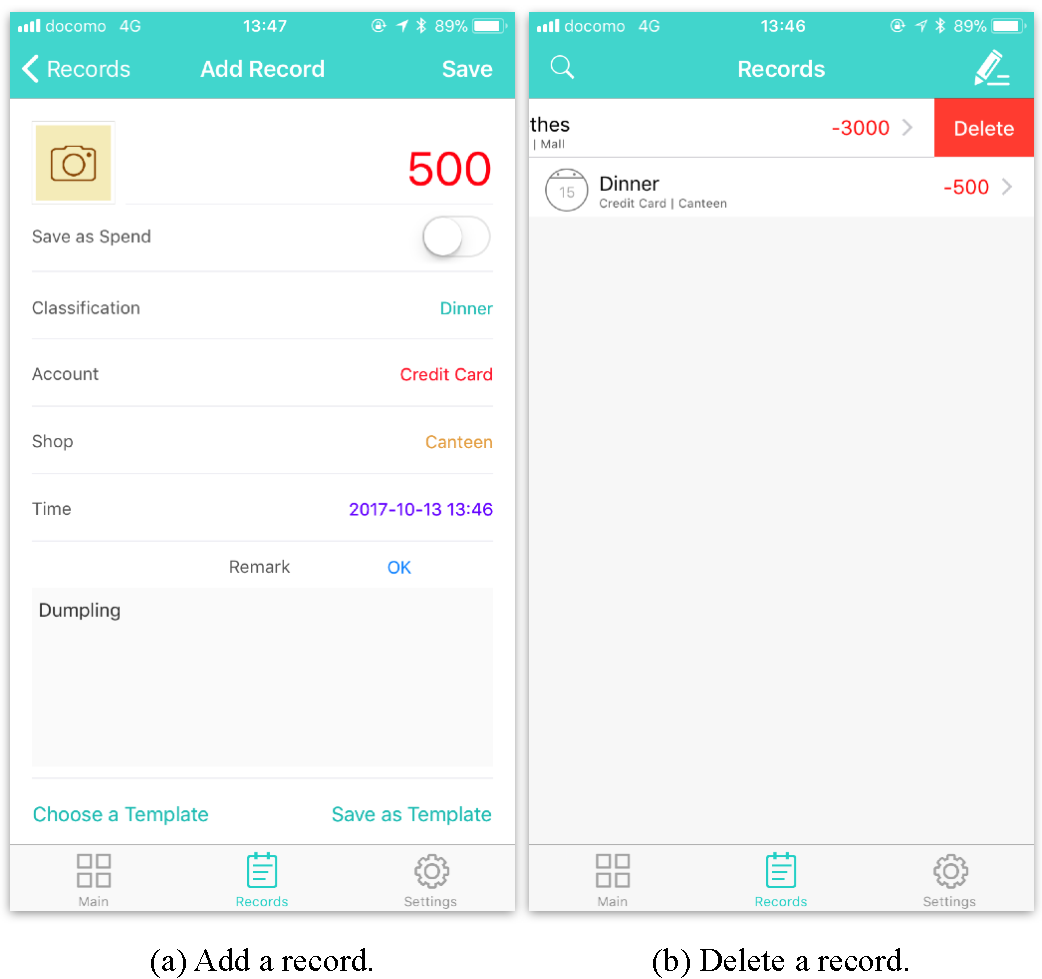
\includegraphics[scale=0.5]{account_book}
	\caption{Screenshots of demo application Account Book.}
\end{figure}

Using the Grouper framework, we have developed the following applications. 

\begin{itemize}
	\setlength{\itemsep}{1pt}
	\setlength{\parskip}{0pt}
	\setlength{\parsep}{0pt}
	\item \emph{Account Book}, an iOS application in Objective-C, records the income and expenditure of a group.
	\item \emph{Test}, a benchmark iOS application in Swift, tests the performance of Grouper.
\end{itemize}

Figure 4(a) shows the screenshot of adding a record in Account Book. 
A user uses Account Book to add income and expenditure records that include classifications, accounts, shops, times and remarks of a group. 
When the user click the save button, Account Book invokes the $grouper.sender.update(object)$ method of Grouper to share this record to other group members.
Figure 4(b) shows the screenshoot of deleting a record in Account Book. 
A user swipes a cell from right to left to delete a record in the record list. 
When the user click the delete button, Account Book invokes the $grouper.sender.delete(object)$ method of Grouper to delete this record on the devices of other group members.

\begin{figure*}[t]
	\centering
	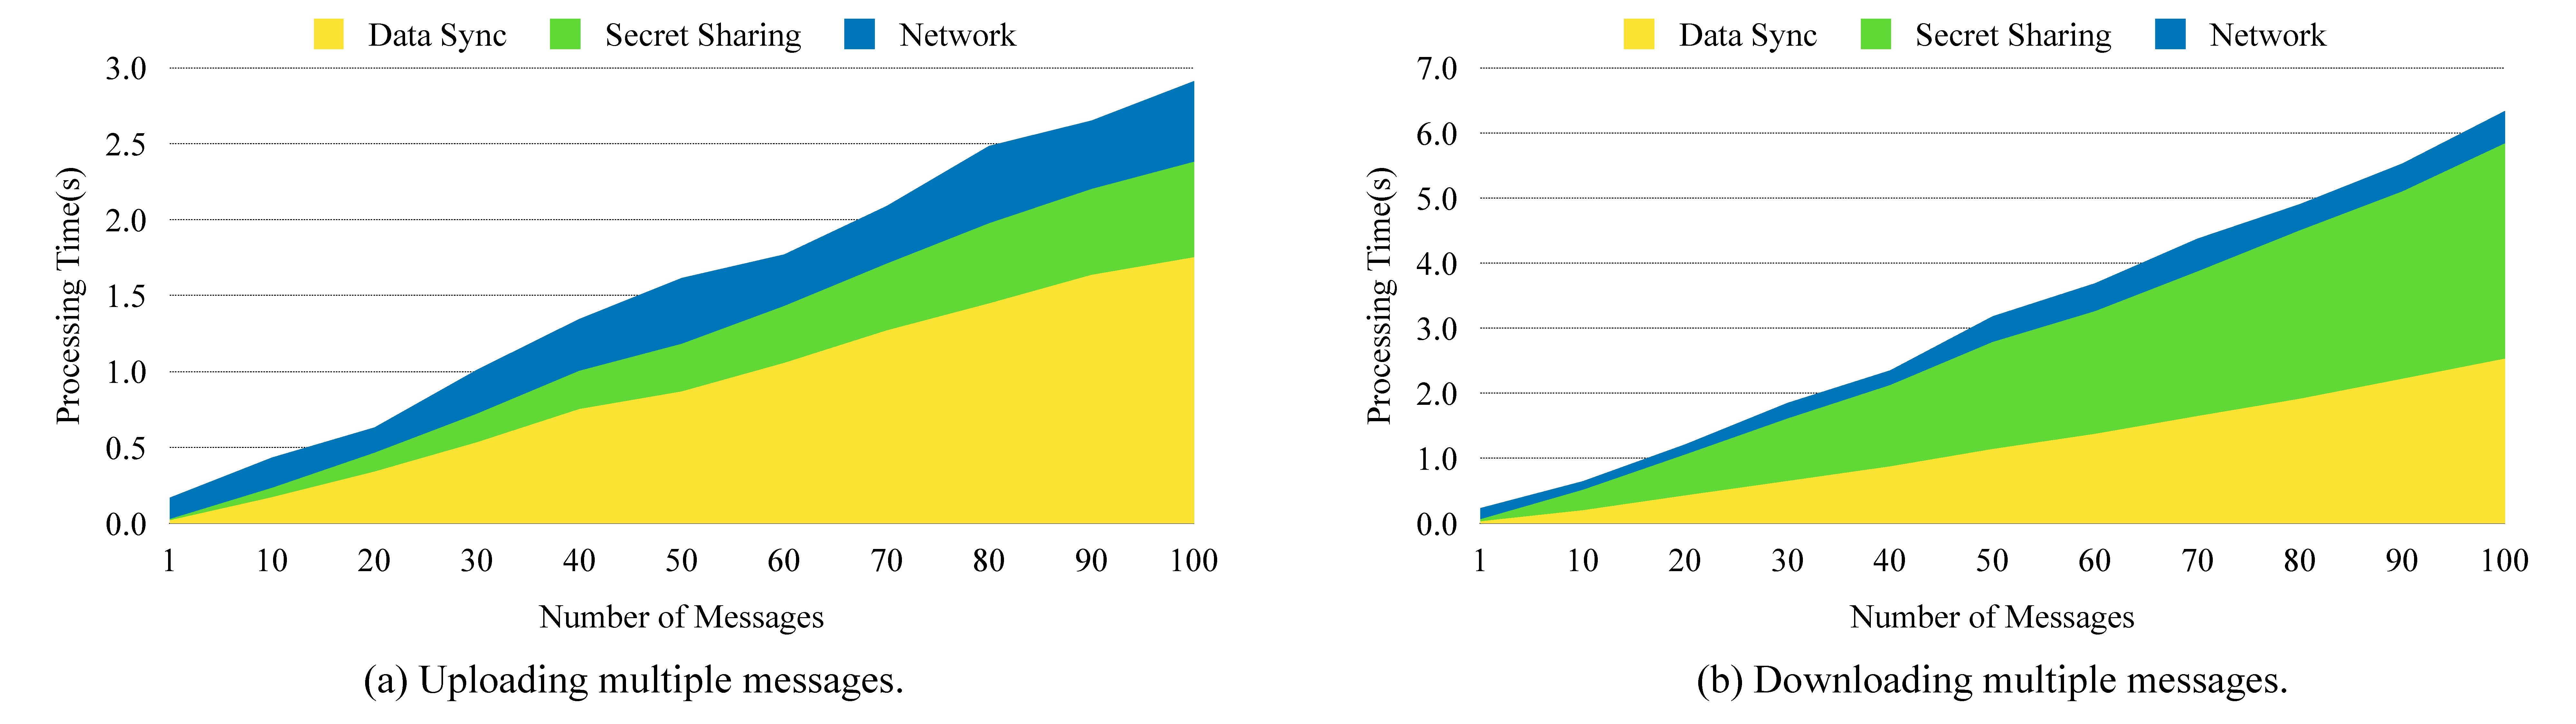
\includegraphics[scale=0.13]{multiple_messages}
	\caption{Processing time of uploading and downloading multiple messages.}
\end{figure*}

\begin{figure*}[t]
	\centering
	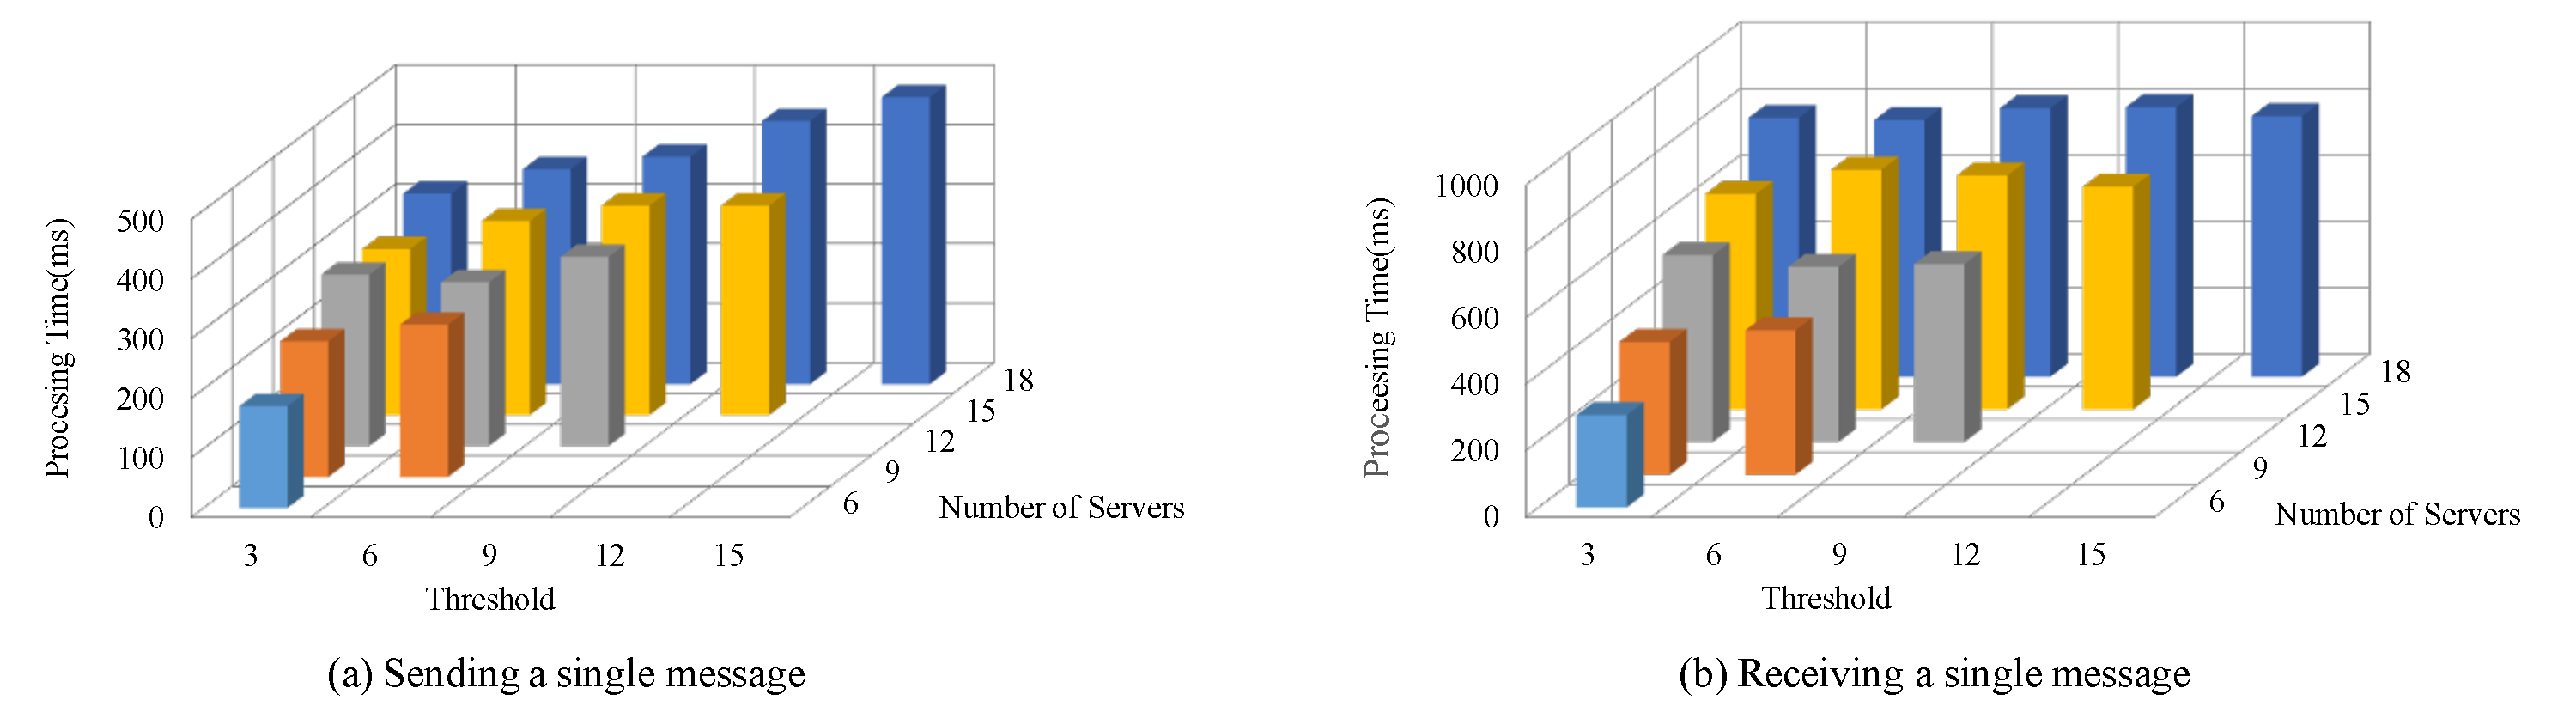
\includegraphics[scale=0.35]{3d}
	\caption{Processing time of uploading and downloading a single message with different scheme.}
\end{figure*}

\begin{figure*}[t]
	\centering
	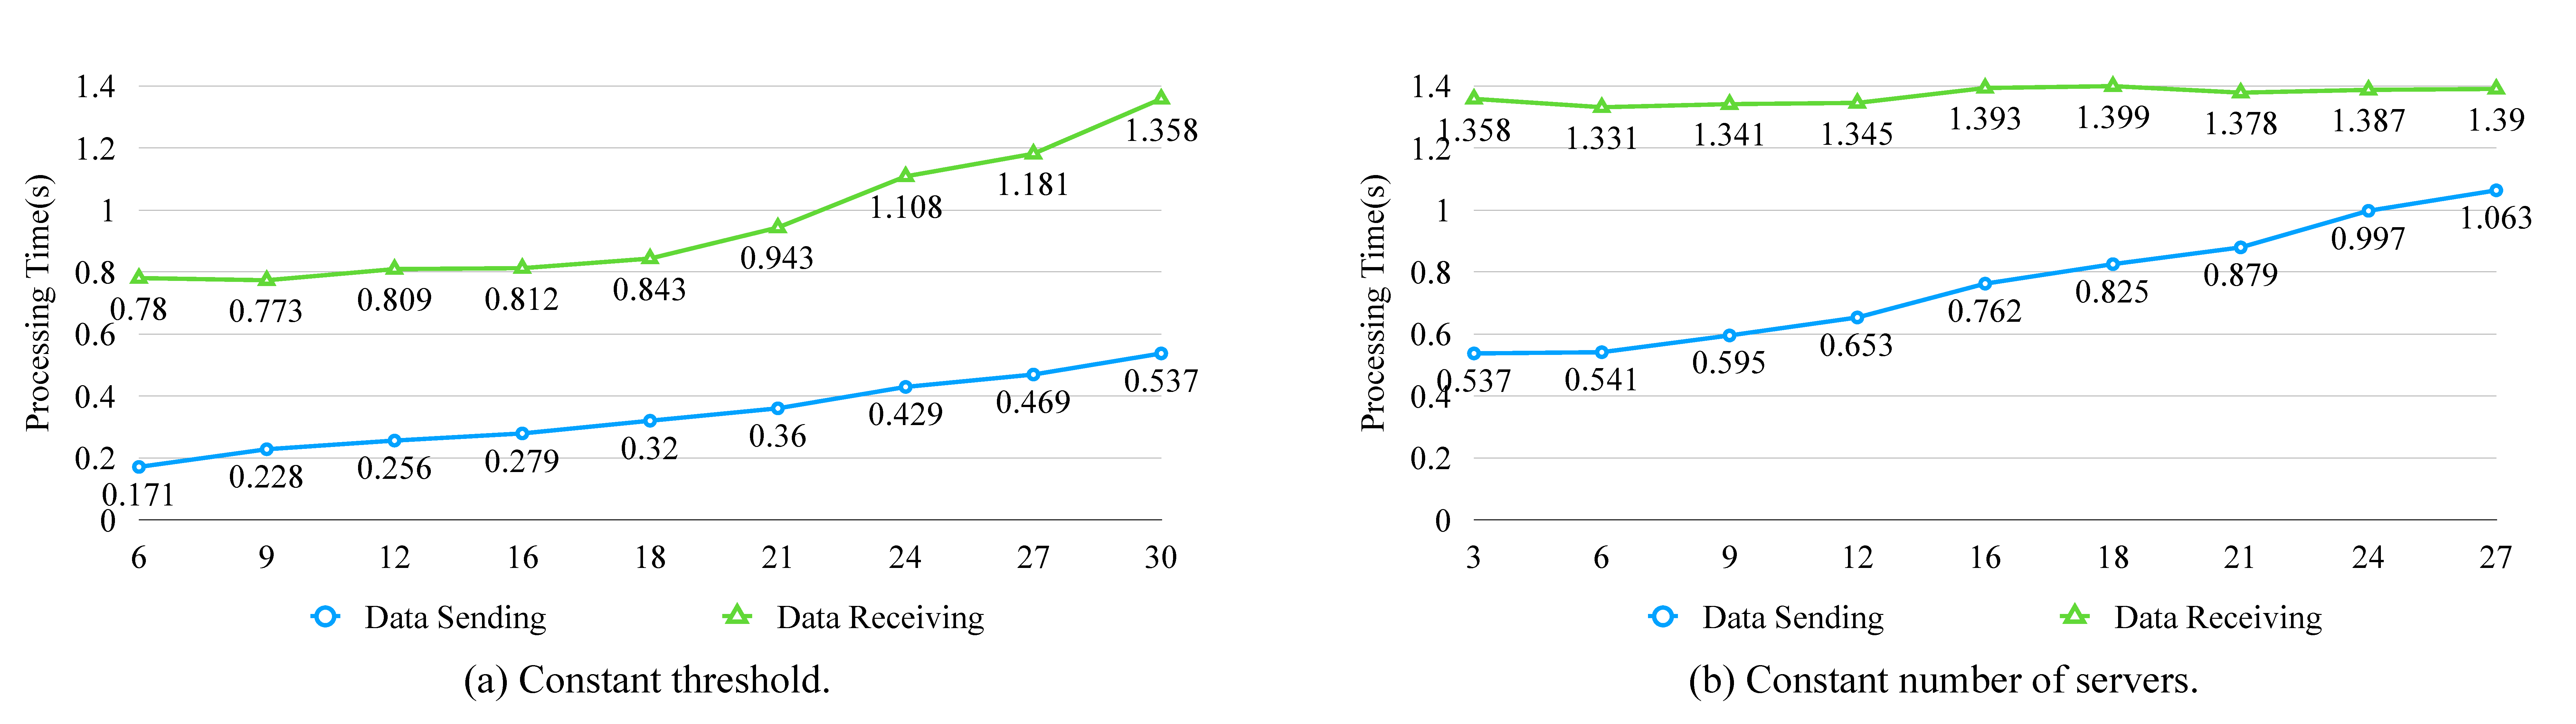
\includegraphics[scale=0.13]{constant_k_n}
	\caption{Processing time of uploading and downloading a single message with a constant ${k}$ or ${n}$.}
\end{figure*}

\section{Evaluation}

This section shows the development efforts to use Grouper and the performance of Grouper.

\subsection{Development Efforts}

We see development efforts through two factors: the usability of the client API and the code size in the lines of code(LoC) the developer has to add after using Grouper. 
As described in Table 1, Grouper provides the simple client APIs for developers.
A developer can convert a standalone application to a data sharing application with our client APIs easily.

To know the LoC developer has to add, we have developed the following applications, Account Book and Test using the Grouper framework.
As described in Table 4, based on the stand alone application without data synchronization, developers can add data synchronization to these applications with Grouper by adding a small number of code. 

\subsection{Performance}

In this subsection, we show that Grouper mobile applications using the Grouper framework provide sufficient performance for small groups of people.
In our performance experiments, we used the benchmark application \emph{Test} to transfer data between iPhone 4s and iPod 5 generation on a wireless LAN network (802.11n).
We installed 30 Web services on three different servers.
Each server ran a Tomcat server instance which hosted 10 Web services.
Table 5 shows the hardware and software information of our experiment environment.
In our benchmark application, the size of an object was about 323 bytes.
This object corresponds to a record of benchmark application Test and contains the creation time of this record.
When this object was updated in a node, the Grouper API generated a normal message which size was about 656 bytes.

\begin{table}[t]
	\footnotesize
	\centering  
	\caption{Devices in the performance experiment.}
	\label{my-label}
	\begin{tabular}{llll}
		\hline
		\textbf{Device} & \textbf{CPU} & \textbf{RAM} & \textbf{OS} \\ \hline
		iPod 5 & A5 & 512MB & iOS 9.3.5 \\
		iPhone 4s & A5 & 512MB & iOS 9.3.5 \\
		Server 1 & Core i7-5820K & 32GB & Ubuntu 14.04.5 LTS \\
		Server 2 & Core i7-5820K & 32GB & Ubuntu 14.04.5 LTS \\
		Server 3 & Core i7-5820K & 32GB & Ubuntu 14.04.5 LTS \\ \hline
	\end{tabular}
\end{table}

Through experiments, we measured the following processing times of object synchronization (uploading and downloading).

\begin{itemize}[leftmargin=*]
	\setlength{\itemsep}{1pt}
	\setlength{\parskip}{0pt}
	\setlength{\parsep}{0pt}
	\item \textbf{The processing time according to the number of updated objects (the number of update messages)}.
\end{itemize}

We performed a experiment to measure the processing time of object synchronization according to the number of updated objects.
In this experiment, we set the secret sharing scheme to ${f(2, 3)}$.
We sent multiple messages from a device and received them in another device. 
Concretely, We sent multiple message from iPod to iPhone for three time and from iPhone to generation for three times.
We obtained the average value of these experimental results.

Figure 5 shows the processing time of uploading and downloading multiple messages.
We divide the processing time into three parts: data sync, secret sharing and network.
As the number of messages increased, the data sync and secret sharing part increased linearly. 
The network part increased slowly and sometimes decreased.
On the whole, the total processing time increased linearly.
Compared with uploading messages, downloading messages cost about two times of processing time.
Note that object synchronization is done in a background task.
Note that object synchronization is done asynchronously.
While the Grouper framework is performing object synchronization, user interface of a mobile application never freezes.
A user is not aware of data synchronization.

The number of messages a device has to handle is independent of the number of devices in a group.
For example, consider that a group consists of 100 members and their 100 devices.
When an object is updated in a device, the device has to send a single update message.
The device divides the message into multiple shares, and uploads them to multiple untrusted servers.
This process is independent of the number of devices in a group. 

\begin{itemize}[leftmargin=*]
	\setlength{\itemsep}{1pt}
	\setlength{\parskip}{0pt}
	\setlength{\parsep}{0pt}
	\item \textbf{The processing time according to the parameters of the secret sharing scheme.}
\end{itemize}

We performed a experiment to measure the processing time of object synchronization according the parameters of the secret sharing scheme.
Specifically, we changed the parameter ${k}$  and ${n}$ of the secret sharing scheme and measured the processing time of uploading and downloading a single message.
Figure 6 shows the relationship between processing time and the parameters, where ${0< k < n, k=3i, n=3j+3, 1 \leq i, j \leq 5}$.
For uploading a single message, as the parameter ${k}$ or ${n}$ increased, processing increased linearly.
However, for downloading a single message, as the parameter ${k}$ increased, processing time  changed a little, sometimes decreased.

Figure 7(a) shows the relationship between processing time and the number of servers ${n}$, where ${k=3}$ and ${n = 2, 4, 6, ... , 10}$. 
Figure 7(b) shows the relationship between processing time and the threshold ${k}$, where ${n=30}$ and ${k = 3, 6, 9, ... , 27}$. 
Here, we can answer the third question.
As n increased, the processing time of uploading and downloading increase linearly. 
As k increased, the processing time of uploading increased linearly and that of downloading did not change. 

\subsection{Discussion About the Numbers of Messages}

In this subsection, we discuss the relationship between TTL and the number of messages. 
As describe in Table 6, we define the following parameters.

\begin{table*}[t]
	\centering
	\caption{The parameters for discussing the relationship between TTL and the number of messages.}
	\begin{tabular}{ll}
		\hline
		\textbf{Parameter} & \textbf{Explanation} \\ \hline
		$D$ & Number of devices. \\
		$T$ & Time to live (TTL). \\
		$F$ & Average number of offline devices during TTL. \\
		$L$ & Average online time. \\
		$Ui$ & Number of updated/deleted objects created in the device $i$ during the TTL. \\ 
		$URi$ &  \begin{tabular}{@{}l@{}}
			Number of updated/deleted objects sent from the device $i$ after downloading resend messages \\ during the TTL. \\
		\end{tabular}\\ 
		$U$ & Total number of updated and deleted objects during the TTL. \\ 
		$C$ & Total number of confirm messages during the TTL. \\ 
		$NUi$ & Number of uploading for device $i$. \\
		$NU$ & Total number of uploading. \\
		$NDi$ & Number of downloading for device $i$. \\
		$ND$ & Total number of downloading. \\ \hline
	\end{tabular}
\end{table*}

At first, we consider the situation that all devices are online ($F=0$).
In this situation, the number of uploading for the device $i$ is

\begin{equation}
NUi = Ui + C
\end{equation}

Total number of uploading is the sum $NU$ of $NUi$.

\begin{equation}
NU = \sum_{i=1}^{D} NUi = U + C \cdot D
\end{equation}

A device should not download those messages uploaded by itself.
To simplify the question, we suppose the device downloads those messages uploaded by itself.
Thus, the number of downloading for device $i$ $NDi$ is equal to total number of uploading $NU$.
Total number of downloading $ND$ is the sum of $NDi$.

\begin{equation}
ND = \sum_{i=1}^{D} NDi = NU \cdot D =  (U + C \cdot D) \cdot D
\end{equation}

Equation 1 to 3 shows that for the device $i$ during the TTL, the order of uploading  is $O(U)$, and the order of downloading is $O(U+D)$.
As the number of updated and deleted objects increased, total number of uploading and downloading increased linearly.

Next, we consider the situation that there are offline devices in a group ($F \neq 0$).
In this situation, offline devices send the resend messages when they are online and those devices which saved the updated objects will send update messages to offline devices.
To simplify the question, we suppose that all offline devices should receive the updated messages after they sent the resend message.
It means that any device will not send a same updated object for more than two times.
For the device $i$, the number of those update messages which are sent after downloading the resend message $URi$ is

\begin{equation}
URi = Ui \cdot \frac{L}{T} \cdot F
\end{equation}

Compared to the situation that $F=0$, in this situation, the number of uploading for the device $i$ includes $URi$.
Thus, we get $NUi$, $NU$ and $ND$ where $F \neq 0$.

\begin{equation}
NUi = Ui + C + Ui \cdot \frac{L}{T} \cdot F = Ui \cdot (1 + Ui \cdot \frac{L}{T} \cdot F) + C
\end{equation}

\begin{equation}
NU = \sum_{i=1}^{D} NUi = U \cdot (1 + \frac{L}{T} \cdot F) + C \cdot D
\end{equation}

\begin{equation}
ND = NU \cdot D = \sum_{i=1}^{D} NUi = U \cdot D \cdot (1 + \frac{L}{T} \cdot F) + C \cdot D^{2}
\end{equation}

Equation 4 to 7 shows that for the device $i$ during the TTL, the order of uploading is $O(U \cdot \frac{L}{T} \cdot F)$, and the order of downloading is $O(U \cdot \frac{L}{T} \cdot F + C)$.
As the number of updated and deleted objects, the average number of offline devices during the TTL, and the average online time increased, total number of uploading and downloading increased linearly.

From the discussion above, we get the conclusion that as the TTL increased, the number of resend and update messages decreased, it becomes more convenient for group members to sharing information.

\section{Related Work}

Vanish is a self-destruction system\cite{geambasu2009vanish}. 
Vanish uses Distribute Hash Tables(DHTs) as the back-end storage.
Vanish encrypts a message with a new random key, threads the key to shares using a secret sharing scheme, stores these shares to a public DHT and eliminate the key from the local storage.
The key in Vanish is removed after a period of time, and the encrypted message is permanently unreadable.
Vanish is implemented with OpenDHT\cite{rhea2005opendht} or VuzeDHT\cite{vuzedht} which is controlled by a single maintainer. 
Thus, it not strongly secure due to some Sybil attacks\cite{wolchok2010defeating}. 
In addition, the surviving time of the key in Vanish cannot be controlled by applications. 

To address these issues in Vanish, Zeng et al., propose SafeVanish\cite{zeng2010safevanish} and SeDas\cite{zeng2012sedas}. 
SafeVanish is designed to prevent hopping attacks by extending the length range of the key shares while SeDas extends the idea of Vanish by exploiting the potentials of active storage networks, instead of the nodes in P2P, to maintain the divided secret key. By extending SeDas, Zeng's group proposes CloudSky\cite{zeng2015cloudsky}, a controllable data self-destruction system for untrusted cloud storage. 
In CloudSky, a user can control the surviving time of a message.
Taking advantage of ABE, a user can also define the access control policy.

However, these proposals are not suitable for developing information sharing applications introduced above. 
They are suitable for exchanging immutable messages, while our target applications need to modify a object repeatedly after other devices received the object. 
Although, CloudSky solves the problems about user controllability in Vanish, offline devices cannot download messages after they have been removed from untrusted servers.
In Grouper, offline devices can download such messages by using confirm and resend messages.
A trusted authority is necessary in CloudSky to manage user profiles, while Grouper does not rely on any trusted authority.

Mylar\cite{popa2014building} stores encrypted data on servers, and decrypts this data only in the browsers of users. 
Developers of Mylar use its API to encrypt a regular (non-encrypted) Web application. 
Mylar uses its browser extension to decrypt data on clients. 
Compared to Mylar which is using a single server, Grouper takes advantages of data redundancy provided by the secret sharing scheme.

Sweets\cite{sweets} is a decentralized social networking service (SNS) application using data synchronization with P2P connections among mobile devices. 
Sweets performs data synchronization not only between two online nodes directly but also via common friends' nodes indirectly for offline nodes.
This indirect synchronization uses ABE to realize access control.
Direct synchronization can only be finished during two devices are online at the same time. 
In Grouper, on the other hand, users can synchronize data from multiple untrusted servers anytime.

DepSky\cite{bessani2013depsky} is a system that stores encrypted data on servers and runs application logic on clients.
\emph{Cloud-of-Clouds} is the core concept in DepSky. 
It represents that DepSky is a virtual storage, and its users invoke operations in several individual severs. 
DepSky keeps encrypted data in commercial storage services and do application logic in individual servers.
In Grouper, untrusted servers undertake responsibility of temporarily data storage and message delivery with server-side computation.

Compared with data encryption methods, the secret sharing scheme has following advantages.
Firstly, using a secret sharing scheme does not require key management including generation and distribution.
Data encryption systems like CloudSky always use trusted authorities for key management.
In Grouper, we require all cloud services are untrusted.
Secondly, the secret sharing scheme ensures the data availability in the situation that a small number of untrusted servers are not accessible.
For the $f(k, n, s)$ scheme in Grouper, the original object can be recovered after accessing at least $k$ untrusted servers.
Thirdly, the secret sharing scheme reduces the risk of attack, because the attacker who can access only $k-1$ or less untrusted servers cannot get any information.

\section{Conclusion}

This paper describes Grouper, a framework using a secret sharing scheme and multiple untrusted servers, to develop light-weight information sharing for mobile applications.
In such an application, users can create a group and exchange the information safely via multiple untrusted servers.
Grouper provides two main functions: reliable data synchronization and group management for developing such applications.
Compared to conventional systems, Grouper provides the reliable synchronization and ensures that a member of a group can synchronize data from others after untrusted severs remove data.
Compared to pure data encryption approaches, Grouper improves dependability by using multiple untrusted servers and our extended scheme $f(k, n, s)$.

We implement Grouper's Web service in Java EE and client's framework in Objective-C. 
To evaluate Grouper's design, we have developed applications, \emph{Account Book} and \emph{Test} on the top of Grouper.
Developing these applications shows that Grouper requires little development efforts to convert an stand alone application to data sharing application.
We also evaluated the performance of Groper using our benchmark application.
The results shows that using Grouper in an application does not influence the user experience.

In the future, we would like to support more platforms including Android.

\bibliographystyle{unsrt}
{
	\footnotesize
	\bibliography{ref}
}

\end{document}
